\newpage
\section{Testing e Verifica dell'Adeguatezza}

Il termine \textbf{testing} si riferisce all'eseguire un programma ed osservarne i risultati, andandoli a confrontare con un risultato atteso (si devono quindi avere delle specifiche). Bisogna inoltre definire quante volte è necessario eseguire l'operazione di testing (\textit{testing adequacy}). Un'altra, meno usata, definizione di testing si chiama ``exhaustive testing'', cioè che il sistema viene testato per tutti i possibili input. Vien da sè capire che questo tipo di testing è controverso, poiché non è possibile controllare tutti i possibili input (che sono infiniti, o comunque enormi). Questa controversia è riconducibile all'\textit{halting problem}: può esistere un algoritmo che risponde \textit{si} o \textit{no} rispetto alla terminazione di un programma qualsiasi? \textit{No}.

Quello che si ottiene attraverso la fase di testing è un'approssimazione ottimistica della qualità, ossia attraverso il test viene scelto un numero piccolo di tutti i possibili input (scelti in maniera intelligente). In particolare, si può ottenere: \begin{itemize}
    \item l'identificazione di un bug;
    \item le prove non manifestano bug (è ottimistico concludere che il programma funziona per tutti gli altri input)
\end{itemize}

Un \textit{criterio di adeguatezza} dovrebbe permettere di rispondere ``si'' o ``no'' alla domanda ``L'insieme di casi di test progettati è sufficiente?'' Può quindi essere visto come un predicato che è \textit{vero} (soddisfatto) o \textit{falso} (non soddisfatto) di una coppia del tipo \texttt{<programma, test suite>}.

\subsection{Terminologia dei bug (IEEE)}

Il termine \textit{bug} ha varie sfumature: \begin{itemize}
    \item failure; \\ osservazione del problema, ma non il codice che l'ha causato. In questa fase, ancora non si sa come correggere il problema
    \item fault; \\ si analizza il malfunzionamento, si analizza il codice, si evidenzia il problema e si comprende come correggerlo
    \item error; \\ ulteriore analisi del fault: ci si chiede il perché si è verificato l'errore, e di conseguenza ci permette di classificare i fault in base all'area in cui appartengono (es. errori di gestione della memoria, etc...)
\end{itemize}

\subsection{Selezionare il test da una failure}

Come abbiamo detto in precedenza, non è possibile testare il software con tutti i possibili input. Come prima cosa, si fanno delle prove che vanno a stimolare il sistema in maniera mirata per trovare delle failure. Questo primo obiettivo è abbastanza intuitivo. Come seconda cosa, mano a mano che vengono eseguiti i test, che vengono identificati bug (e corretti), i pochi test rimasti da fare vano in convergenza. In pratica, una volta verificato che il software supera tutti i test previsti, ci si chiede \textit{``cosa sappiamo?''} In particolare, ci chiediamo se i test che abbiamo fatto siano sufficienti per poter definire il software di qualità e pronto al rilascio.

Le fasi, riassumendo, sono due: \begin{enumerate}
    \item effettuare prove intelligenti mirate alla risoluzione dei bug;
    \item verificare che le prove scelte nel punto precedente siano anche adeguate.
\end{enumerate}

\begin{example}{}{Simple game}
    Consideriamo la seguente applicazione sulla quale vogliamo eseguire dei test:

    \begin{figure}[H]
        \caption{Simple Game}
        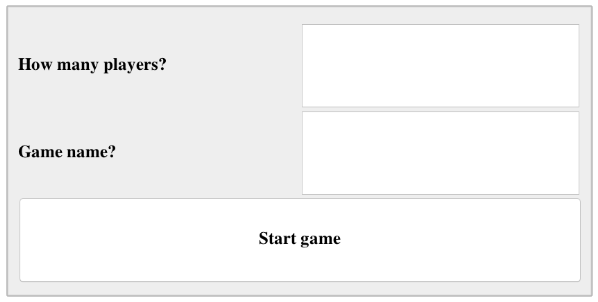
\includegraphics[width=\textwidth]{Lezioni/Lezione2/simplegame.png}
    \end{figure}

    L'applicazione è dotata di due campi di testo (numerici o testuali) ed un pulsante per far partire il sistema. È bene sottolineare che non si vuole entrare nei dettagli specifici del programma, ma semplicemente si vuole lavorare sula base dell'interfaccia data.

    Il programma, per avviare il gioco, richiede di specificare il numero di giocatori ed il nome della partita. Il tasto ``Start game'' deve avviare il gioco in maniera corretta.

    Effettuare il testo di questa applicazione vuol dire inserire dei valori nei campi specificati, premere ``Start game'' ed osservare il comportamento in modo da verificarne la correttezza. Si richiede di scegliere al più \textit{dieci} prove da effettuare:

    \begin{figure}[H]
    \caption{Casi per Simple Game}
    \begin{center}
    \begin{tabular}{c | > {\centering}p{7cm} | c}
        Caso standard  & \centering Casi di errore previsto & Casi di stress \\ \hline
        Players $\geq 1$ & Nome con caratteri particolari potrebbero mandare in crash il sistema & Players molto elevato \\
        & Players con lettere invece di numeri & Nome stringa lunga \\
        & Players < 0 & \\
        & Campi vuoti & \\
        & Players è un double & \\
    \end{tabular}
    \end{center}
    \end{figure}
    Si può osservare che si sono considerati i casi in cui il sistema potrebbe andare in crash (lo sviluppatore non è stato attento).
\end{example}

\subsection{Test Obligations e Test Cases}

Quando si ragiona sull'identificazione dei test, vengono identificati una serie di elementi (come nell'esempio sopra) che vengono indicati come ``test objectives'' o ``test obligations''.

Se non si conosce la specifica del sistema, si possono individuare casi di crash/malfunzionamento che si verificano per qualunque sistema, indipendentemente dal dominio applicativo. Tuttavia, molti fallimenti dipendono dal sistema, pertanto, quando si passa all'obiettivo del test alla corrispondente implementazione, si ha che quest'ultima è fatta dai risultati attesi degli stessi. Per conoscere questi risultati attesi, è \textit{necessario} conoscere la specifica del sistema.

\begin{itemize}
    \item \textbf{Test Obligations}: test che devono essere effettuati almeno una volta per verificare il corretto funzionamento dell'applicazione. Non è necessario conoscere la specifica;
    \item \textbf{Test Case}: test fatti ad-hoc per dei casi particolari. È necessario conoscere la specifica \textit{prima} di eseguire il test.
\end{itemize}

\begin{example}{}{Simple Game - Specifica}
    \begin{quotation}
    L'applicazione (\textit{Simple Game}) permette all'utente di creare delle istanze di un gioco. Per creare tali istanze è necessario specificare il numero di giocatori e un nome della partita. Il gioco richiede almeno cinque giocatori ed al massimo può essere giocata da trenta giocatori. Se i giocatori sono più di trenta, allora il gioco parte comunque, ma in una modalità specifica denominata ``Team-Mode''. Il gioco può partire in modalità ``Private-Mode'' se il nome del gioco comincia con l'asterisco, oppure in ``Public-Mode'' se non comincia con l'asterisco (quindi in tutti gli altri casi).
    \end{quotation}

    Questo è un esempio di specifica della nostra applicazione. È pertanto possibile definire dei valori per il valore atteso di ciascun obiettivo.

    Supponiamo di considerare l'input seguente:

    \begin{itemize}
        \item Players = 5
        \item Name = ``nome''
    \end{itemize}

    Secondo la specifica, è possibile dedurre i valori attesi:

    \begin{itemize}
        \item Con 5 giocatori il gioco può partire in modalità normale
        \item Con ``nome'' il gioco partirà in ``Public-Mode'' in quant il nome non contiene un asterisco
    \end{itemize}

    Chiaramente, se il valore atteso corrisponde a quello del valore ottenuto con l'input specificato, allora il test ha avuto successo, altrimenti avremo un \textit{bug}.

    Quindi, alla luce della specifica sopra introdotta, è facile vedere come gli obiettivi di test prima individuati non siano più ottimali.

    \begin{figure}[H]
    \caption{Casi per Simple Game dopo la specifica}
    \begin{center}
    \begin{tabular}{c | > {\centering}p{5cm} | c}
        Caso standard  & \centering Casi di errore previsto & Casi di stress \\ \hline
        Players $\geq 5$ & Campi vuoti & Players molto elevato \\
        Players $\geq 5$ e $\leq 30$ & Players $<$ 5 & \\
        Nome con ``*'' & & \\
        Nome senza ``*'' & & \\
        Nome = ``*'' & & \\
        Nome con ``*'' in mezzo & & \\
        Nome con ``*'' e spazio & &
    \end{tabular}
    \end{center}
    \end{figure}

    Lo stesso obiettivo di test può essere raggiunto da più valori (considerando l'esempio precedente, è possibile provare l'applicazione per Players = 40, Players = 32, etc...).

\end{example}

\subsection{Boundary Testing}

Fino ad ora non abbiamo però tenuto conto dei cosiddetti \textit{casi limite} o \textit{boundary testing}, ossia i test effettuati usando valori che soddisfano una casistica molto specifica, che nel nostro esempio per ``Simple Game'' possono essere Players = 5, Players = 30, Players = 31.

La specifica distingue una serie di comportamenti, di cui tre risultano essere particolarmente di interesse:
\begin{itemize}
    \item Players = 5 \\ Il gioco non funziona
    \item Players = 30 \\ Il gioco funziona in modalità non a squadre
    \item Players = 31 \\ Il gioco funziona in ``Team-Mode''
\end{itemize}
Questi comportamenti dipendono dal parametro \textit{numero di giocatori}, tuttavia, sono adiacenti l'uno all'altro (c'è un valore specifico per il quale ad un certo punto si passa da un comportamento ad un altro). Il comportamento del sistema è quindi \textit{non-lineare}.

In generale quindi, si cercano di identificare tre cose: \begin{enumerate}
    \item Comportamenti normali \\ Esplicitamente definiti dalla specifica
    \item Comportamenti eccezionali \\ Implicitamente suggeriti dalla specifica, e sono di ``contorno'' ai comportamenti normali
    \item Casi di confine
\end{enumerate}

I comportamenti individuati nel nostro sistema di esempio sono: \begin{enumerate}
    \item Comportamenti normali \begin{itemize}
        \item Players < 5
        \item Players $\geq 5$ e $\leq 30$
        \item Players > 30
    \end{itemize}
    \item Comportamenti eccezionali \begin{itemize}
        \item Players è una stringa (dovrebbe essere un numero)
        \item Name è una stringa vuota (campo non compilato)
    \end{itemize}
    \item Casi di confine \begin{itemize}
        \item Players = 4
        \item Players = 5
        \item Players = 30
        \item Players = 31
    \end{itemize}
\end{enumerate}